%% derived from https://tex.stackexchange.com/questions/357538/graph-of-a-parabola-on-pgfplots
%% Thanks to Stefan Pinnow
%%     https://tex.stackexchange.com/users/95441/stefan-pinnow

\begin{figure}
  \centering
  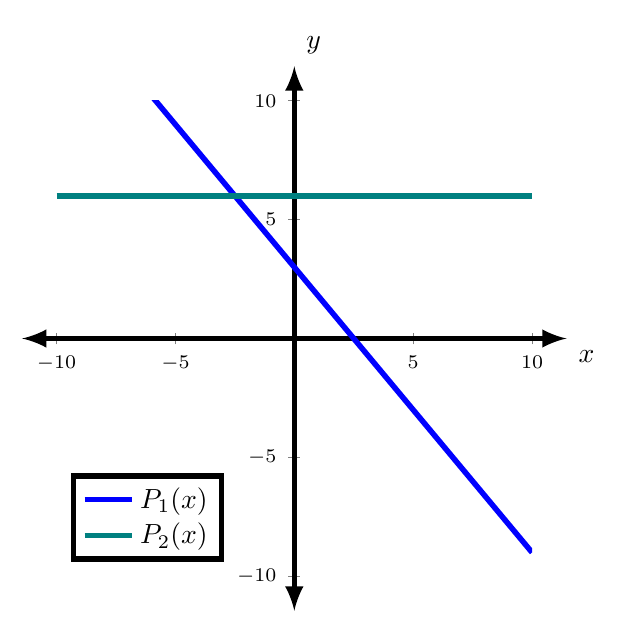
\begin{tikzpicture}
    \begin{axis}[
        legend pos=south west,
        samples=51,
        smooth,
        domain=-10:10,
        line width=2pt,
        width=3in,
        height=3in,
        axis lines=middle,
        xmin=-10,
        xmax=10,
        ymin=-10,
        ymax=10,
        scaled ticks=false,
        ticklabel style={font=\scriptsize},
        xlabel=$x$,
        ylabel=$y$,
        axis line style={
          latex-latex,
          shorten >=-12.5pt,
          shorten <=-12.5pt,
        },
        xlabel style={at={(ticklabel* cs:1)}, xshift=12.5pt, anchor=north west},
        ylabel style={at={(ticklabel* cs:1)}, yshift=12.5pt, anchor=south west},
      ]
      \addplot[color=blue] {-1.2*x + 3};
      \addlegendentry{\(P_1(x)\)}
      \addplot[color=teal] {6};
      \addlegendentry{\(P_2(x)\)}
    \end{axis}
  \end{tikzpicture}
  \caption{Line: $y = P(x) = -1.2*x + 3$}
  \label{fig.line}
\end{figure}
